
\chapter{Reconnaissance basée sur les réseaux convolutifs}

L'une des méthodes les plus efficaces pour la reconnaissance 
d'image est basée sur des réseaux convolutifs. 
Il s'agit de réseaux de neurones profonds où les neurones 
d'une couche à la suivante ne sont pas forcément tous connectés, 
notamment dans les premières couches.
Sur ces couches, l'image d'entrée est découpée en zones que l'on 
appelle tuile ou \nfw{patch}, qui peuvent ou non se chevaucher.
Ces \nfw{patch} sont traités séparement par des neurones qui 
y appliquent des fonctions particulières au traitement d'image
(on parle de traitement convolutif).
Ce n'est que dans des couches plus profondes que les résultats 
sont "agglomérés" pour obtenir une prédiction.

On décompose le problème en plusieurs étapes:
\begin{enumerate}
  \item création du modèle de réseau convolutif, on définit le nombre de 
  couches et les caractéristiques de chaque couche;
  \item entraînement, on utilise les données d'entraînement pour modifier les 
  poids du réseau;
  \item évaluation de l'\nfw{accuracy} du réseau, on utilise le jeu de test 
  pour évaluer les performances de notre réseau;
  \item prédiction, on utilise notre réseau entraîné pour faire des prédictions.
\end{enumerate}

En plus de cela, il est possible d'évaluer la qualité de notre modèle (défini 
à l'étape 1) par validation croisée. 
On découpe le jeu d'entraînement en $k$ groupes et on utilise $k-1$ groupes 
pour effectuer l'entraînement et le dernier groupe pour évaluer le réseau (taux 
de reconnaissance). 
On répète l'opération en utilisant chacun des groupes une fois pour l'évaluation.
En effectuant plusieurs fois l'opération de découpage en $k$ groupes, on 
est en mesure d'obtenir une valeur moyenne pour la précision ainsi qu'une variance. 



\section{Construction du réseau et description des différentes couches}

Nous avons utilisé la bibliothèque \Python \tcode{keras} pour construire 
le réseau convolutif. 
Le code correspondant à la création du modèle est très simple avec cette 
bibliothèque.

\begin{codeblock}
def build_classifier():
    classifier = Sequential()
    classifier.add(Conv2D(32, (3, 3), input_shape=(28, 28, 1), activation='relu'))
    classifier.add(MaxPooling2D(pool_size=(2, 2)))
    classifier.add(Conv2D(32, (3, 3), activation = 'relu'))
    classifier.add(MaxPooling2D(pool_size=(2, 2)))
    classifier.add(Flatten())
    classifier.add(Dropout(0.1)) 
    classifier.add(Dense(units = 128, activation='relu'))
    classifier.add(Dropout(0.1)) # Overfitting reduction - Dropout
    classifier.add(Dense(units = 10, activation='softmax'))
    classifier.compile(loss='categorical_crossentropy', optimizer='adam', metrics=['accuracy'])
    return classifier
\end{codeblock}

Nous allons faire une description ligne à ligne du code précédent.

\begin{codeblock}
classifier = Sequential()
\end{codeblock}

Cette ligne indique que l'on souhaite utiliser un modèle séquentiel, 
c'est à dire un modèle où les couches du réseau sont parcourues linéairement, 
les unes après les autres.

\begin{codeblock}
classifier.add(Conv2D(32, (3, 3), input_shape=(28, 28, 1), activation='relu'))
\end{codeblock}

On ajoute à notre réseau une première couche dite de convolution. 
Comme il s'agit de la première couche, on doit préciser la dimension de 
l'\nfw{input}. 
Ici, nos images seront des tableaux de $28 \times 28$ pixels.  
L'opération de convolution consiste à appliquer des filtres à nos images. Ce type 
d'opération est notamment utilisé en traitement d'image pour appliquer une fonction
particulière à une image. Par exemple, le filtre moyenne remplace chaque pixel par la 
moyenne des pixels adjacents et du pixel central. Ce filtre peut etre utilisé par
exemple pour réduire le bruit. De la même manière il existe des filtres de détection de 
contours ou encore des filtres mettant en avant les changements brutaux de luminosité.

\begin{figure}[h]
  \centering
  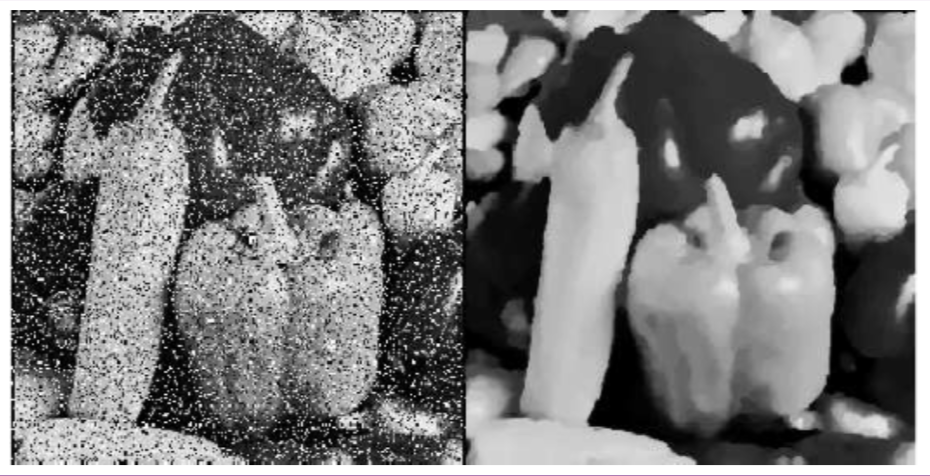
\includegraphics[scale=0.3]{assets/filtre-moyenne}
  \caption{Filtre moyenne.}
  \label{fig:filtre_moyenne}
\end{figure}

Mathématiquement, appliquer un filtre à une matrice de pixels consiste à effectuer le 
produit scalaire d'une portion de l'image par une matrice de petite taille (ici 
$3 \times 3$). Le principe de cette opération est que les portions de l'image sur 
lesquelles sont appliquées ces produits scalaires se chevauchent. Ainsi l'information 
locale est préservée et on garde la cohérence de l'image.

\begin{figure}[h]
  \centering
  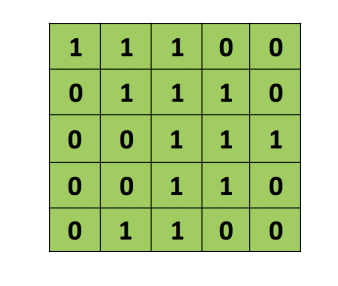
\includegraphics[scale=0.5]{assets/matrice-pixels}
  \caption{Matrice à filtrer.}
  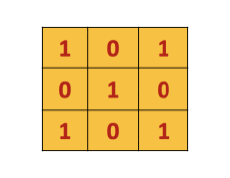
\includegraphics[scale=0.5]{assets/filtre}
  \caption{Exemple de filtre.}
  \label{fig:filtre}
\end{figure}

\begin{figure}[h]
  \centering
  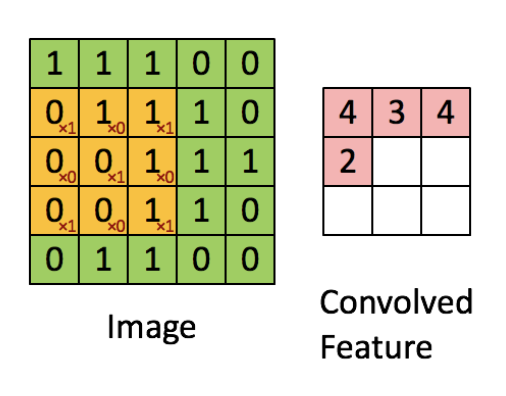
\includegraphics[scale=0.6]{assets/filtrage}
  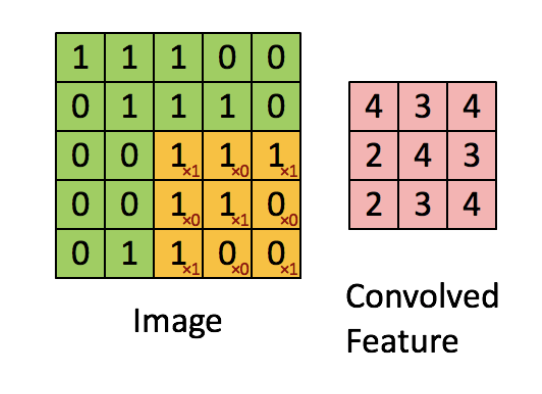
\includegraphics[scale=0.6]{assets/image-filtree}
  \caption{Filtrage de l'image.}
  \label{fig:filtrage}
\end{figure}


On précise également une fonction d'activation qui est ici \tcode{relu}.
Les fonctions d'activation permettent de transformer le signal 
entrant en signal de sortie. On peut citer notamment les 
fonctions tangante hyperbolique, sigmoïde, exponentielle. La fonction d'activation 
\tcode{relu} est la plus populaire dans le cadre des réseaux de neurones à convolution.
Les deux premiers arguments sont les plus intéressants. 
On indique que l'on souhaite appliquer $32$ filtres à des \tcode{patch} de taille 
$3 \times 3$. 

\begin{figure}[h]
  \centering
  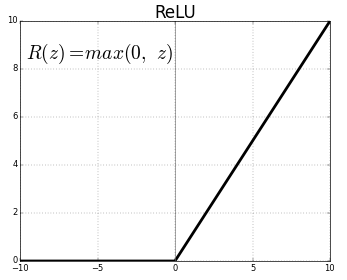
\includegraphics[scale=0.35]{assets/reLu}
  \caption{fonction d'activation reLu.}
  \label{fig:reLu}
\end{figure}

Comme l'on ne précise rien d'autre, les \tcode{patch} se chevauchent par défaut avec un 
décalage de 1. 
On obtient donc en sortie de cette couche une image de taille $26 \times 26$ pour 
chacun des 32 filtres soit $26 \times 26 \times 32$ valeurs.

\begin{codeblock}
classifier.add(MaxPooling2D(pool_size=(2, 2)))
\end{codeblock}

\begin{figure}[h]
  \centering
  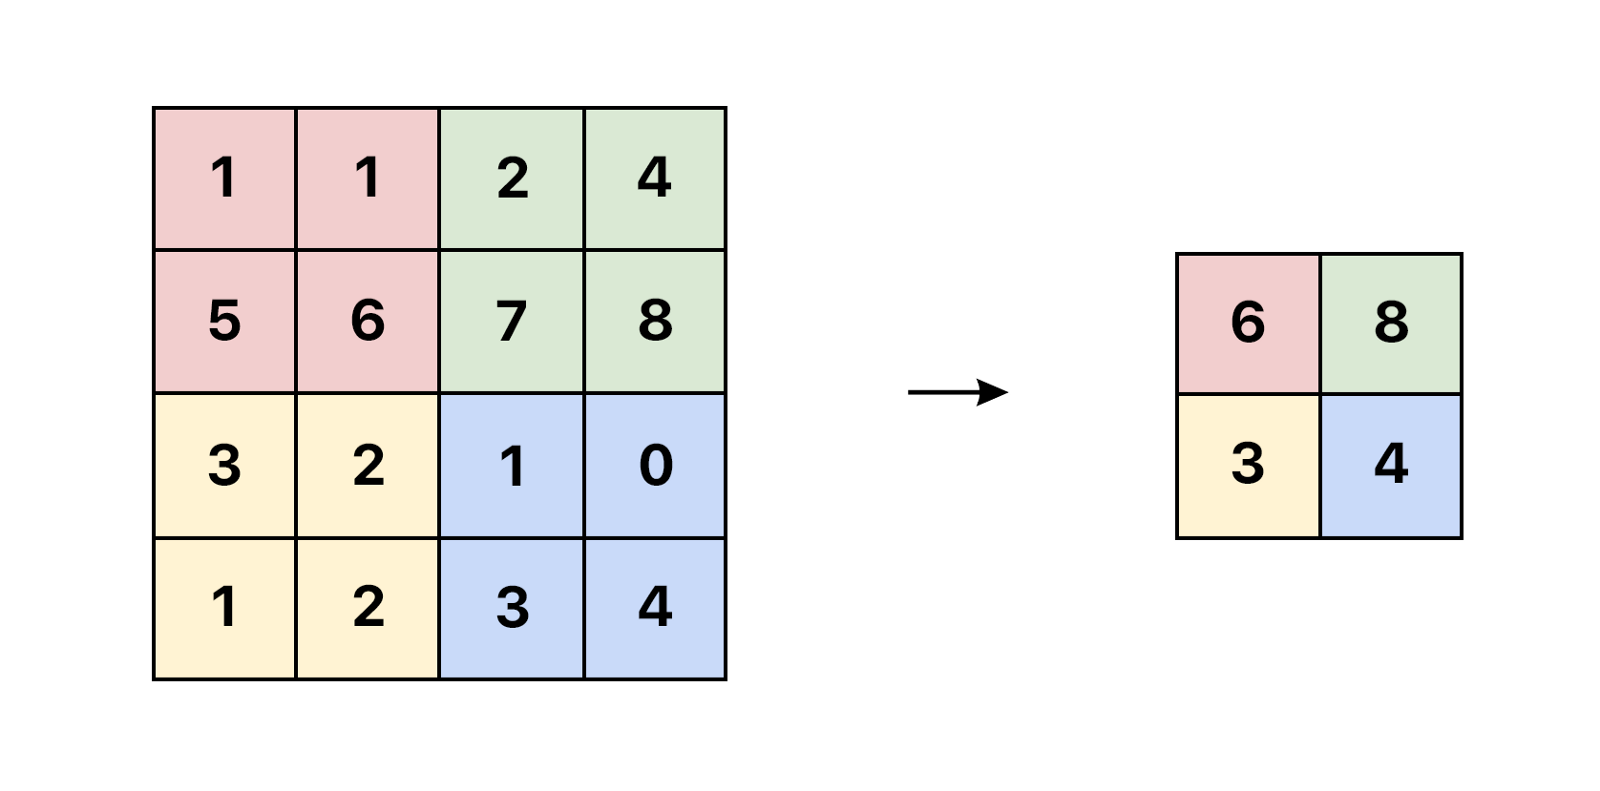
\includegraphics[scale=0.2]{assets/pooling}
  \caption{Max pooling operation.}
  \label{fig:pooling}
\end{figure}

On applique dans cette couche une fonction à des \tcode{patch} de taille $2 \times 2$ 
qui ne se chevauchent pas. 
Le Pooling est une méthode permettant de réduire la taille d'une image tout en préservant 
les informations essentielles. Cette opération permet aussi de réduire le 
sur-apprentissage en généralisant l'information localement.
Comme le suggère le nom, la fonction appliquée ici est \tcode{max}. C'est la méthode
de pooling la plus courante mais il existe de même des méthodes de pooling utilisant 
les fonctions \tcode{average} ou \tcode{median} par exemple. 
Nos images de taille $26 \times 26$ voient donc leur taille réduite de moitié. 
On garde cependant une image pour chaque filtre de la première convolution 
soit un espace de sortie de taille $13 \times 13 \times 32$.

Notons que l'on a plus besoin de préciser la taille de l'entrée dans cette 
couche (elle est déduite automatiquement de la couche précédente).

\begin{codeblock}
classifier.add(Conv2D(32, (3, 3), activation = 'relu'))
\end{codeblock}

On réapplique ici une seconde couche de convolution soit 32 filtres en utilisant des 
\nfw{patch} de taille $3 \times 3$. 
Les images de sortie auront donc une taille de $11 \times 11$ et on obtient donc une 
sortie de taille $11 \times 11 \times 32$ (chacun des 32 filtres n'est ici appliqué qu'à 
une seule image).

\begin{codeblock}
classifier.add(MaxPooling2D(pool_size=(2, 2)))
\end{codeblock}

On refait un \tcode{MaxPooling2D} ce qui réduit la taille de la sortie 
à $5 \times 5 \times 32$. En effet lorsqu'une zone n'est pas recouverte entièrement par 
un patch, celle-ci n'est pas prise en compte (cf. zone grisée de la figure suivante).

\begin{figure}[h]
  \centering
  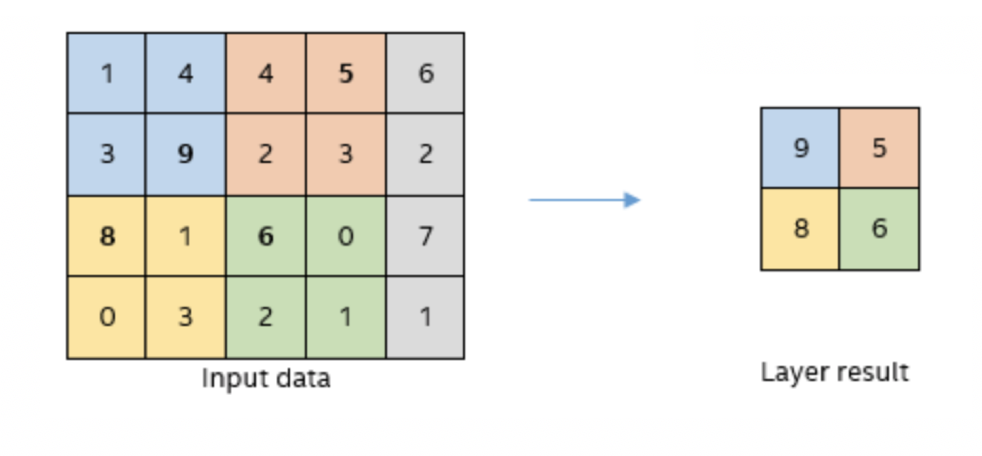
\includegraphics[scale=0.5]{assets/max-pooling-reduced}
  \caption{Max pooling avec zone non prise en compte.}
  \label{fig:max-pooling-reduced}
\end{figure}

\begin{codeblock}
classifier.add(Flatten())
\end{codeblock}

On ajoute alors une couche qui aplatit la sortie de la couche précédente : cette étape est 
nommée flattening.
On obtient donc un vecteur de taille $800$.


\begin{codeblock}
classifier.add(Dropout(0.1)) 
\end{codeblock}

Cette ligne de code supplémentaire permet de mettre aléatoirement à zéro une partie des 
inputs de notre réseau pendant l'entraînement pour limiter le sur-apprentissage. Ici 10\%
des entrées sont mises à zéro.

\begin{codeblock}
classifier.add(Dense(units = 128, activation='relu'))
\end{codeblock}

On ajoute enfin une couche de neurones \nfw{fully-connected}. 
Cela correspond à une couche classique d'un réseau de neurones telle que présentée 
dans la section \ref{reseau}. 
On précise la dimension de l'espace de sortie, $128$; et la fonction 
d'activation, \tcode{relu}. 

\begin{codeblock}
classifier.add(Dropout(0.1)) 
\end{codeblock}

Une autre couche de \nfw{dropout} !


\begin{codeblock}
classifier.add(Dense(units = 10, activation='softmax'))
\end{codeblock}

La dernière couche du réseau, ayant 10 sorties correspondant à nos 10 classes. 
La fonction d'activation utilisée ici est \tcode{softmax}. 
Cette fonction permet de transformer un vecteur de nombres positifs en 
un vecteur définissant une probabilité (les composantes peuvent être 
vues comme la probabilité d'appartenance à la classe associée).
    
	
\begin{codeblock}
classifier.compile(loss='categorical_crossentropy', optimizer='adam', metrics=['accuracy'])
\end{codeblock}

On compile notre modèle, on peut désormais entraîner notre réseau. 
Il reste cependant un certain nombre de paramètres à régler pour optimiser notre modèle.

\section{Optimisation du modèle}

\subsection{Paramètres du modèle}

Les principaux paramètres du modèle sont :

\begin{itemize}
\item Batch size : les images ne sont pas propagées dans le réseau une par une mais par 
paquets ou batch. Ce paramètre détermine donc la taille de ces paquets. Les poids du réseau
sont mis à jour après le passage de chacun de ces paquets. Typiquement plus le batch size
est petit meilleur sera l'apprentissage. En revanche le temps de calcul est alors d'autant
plus long. Un bon compromis consiste souvent à prendre ce paramètre égal à 32.
\item Nombre d'epochs : comme précisé plus haut, un epoch correspond à un passage au travers du réseau de 
l'ensemble des données d'entrainement. Pour continuer d'enrichir le modèle, ce processus 
est répété plusieurs fois. La précision du modèle augmente donc avec le nombre d'epochs 
jusqu'à un certain point de stagnation. 
\item Optimizer : il s'agit de l'algorithme mettant à jour les poids par rétro-propagation.
Les optimizer les plus populaires sont le classique stochastic gradient descent, adam et
rmsprop. Certains algorithmes sont plus adaptés à certains types de réseau. 
\item Le nombre de couches, leur agencement, ainsi que les paramètres internes 
à chaque couche tels que le nombre de filtres et leur taille pour la convolution
et la taille des opérateurs de pooling. 
\end{itemize}

Cette dernière partie est la plus complexe à optimiser car contrairement aux premiers 
paramètres cités, les formes de réseaux possibles sont infinies. En effet, s'il est possible 
de déterminer les paramètres optimaux avec une méthode du type GridSearchCV, il n'est en 
revanche pas possible d'établir une méthode pour déterminer le nombre de couches idéal, 
leur ordonnancement et les paramètres associés. C'est ici avant tout l'expérience qui va 
déterminer la configuration à adopter même s'il est possible de tester un certain nombre de
configuration en cross validation. Les data scientist mettent souvent en avant l'importance
de l'intuition dans l'établissement d'un réseau de neurones, notamment pour cette raison.

\subsection{Réduction du sur-apprentissage}

Nous avons déjà vu une méthode essentielle à la réduction du sur-apprentissage avec 
l'utilisation de drop out. Tout comme pour les paramètres des différentes couches, le 
pourcentage de noeuds à aléatoirement mettre à zéro de même que le positionnement de ces
drop out au sein du réseau sont des paramètres qui relèvent de l'expérience et de 
l'expérimentation. 

Cependant, il y a un autre point important sur lequel jouer pour limiter le phénomène de
sur-apprentissage. Il s'agit de détériorer volontairement le jeu de données d'entrainement
par une série de transformations aléatoires telles que des translations, des zooms ou
encore des rotations. Ces légères modifications permettent de rendre le jeu de données 
plus hétérogène et limitent donc certains biais liés à la méthode de création du jeu de
données. Dans le cadre d'enregistrement de nombres manuscrits comme réalisé avec le jeu de 
données MNIST, malgré un effort pour avoir des données les plus variées possible, en faisant
appel à de nombreuses personnes pour la rédaction des caractères, certains biais subsistent.
Par exemple la méthode même de numérisation des données, la qualité globale des images,
le contraste, l'épaisseur du trait, le centrage des caractères sont autant de facteurs qui 
influencent l'apprentissage d'un modèle prédictif. Détériorer intelligemment le jeu de
données initial peut donc apporter une amélioration significative au modèle en limitant 
ces biais mais aussi en enrichissant le modèle. 

Sous \Python \tcode{keras}, la méthode couramment utilisée pour réaliser cette opération
est ImageDataGenerator dont les principaux paramètres sont :

\begin{itemize}
\item rotation_range 
\item width_shift_range, height_shift_range
\item zoom_range
\end{itemize}

La figure suivante illustre l'utilisation
de cette méthode dans le problème classique de classification de photos de chats et de
chiens. 

\begin{figure}[h]
  \centering
  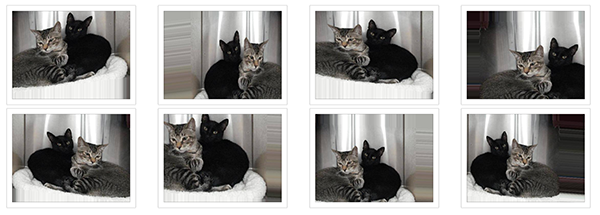
\includegraphics[scale=0.9]{assets/augmented-image}
  \caption{Exemple d'utilisation de ImageDataGenerator}
  \label{fig:augmented-image}
\end{figure}

Dans le cadre de la prédiction de caractères manuscrits, seuls les zooms et 
déformations verticales et horizontales sont intéressants ainsi que les rotations dans une 
certaine mesure (pour imiter l'écriture légèrement penchée de certaines personnes par 
exemple). Les renversements d'image sont ici à proscrire. Ces modifications 
permettent à la fois de faire varier l'épaisseur du trait, le centrage de l'image et 
apportent de la diversité en déformant certains caractères. Il peut aussi s'avérer judicieux
de faire varier les niveaux de gris. Ceci afin de corriger un éventuel biais lié à la 
méthode d'enregistrement mais aussi pour enrichir une fois de plus le jeu de données en 
faisant varier ce que l'on pourrait comparer à l'intensité du trait. Dans le cas de 
l'écriture manuscrite avec un crayon par exemple, plus l'utilisateur appuie fort lorsqu'il 
écrit, plus les niveaux de gris seront élevées après numérisation. De même le type de 
stylo utilisé peut être un facteur limitant pour un modèle entrainé avec des données
très homogènes.
